\section{Grundlagen}\label{grundlagen}
Das erste Kapitel beschäftigt sich mit den Grundlagen, diese sind zum Verständnis der nachfolgenden Kapitel notwendig.
\\
Zuerst wird erläutert, was ein Selbstbedienungsstand ist.
Anschließend wird es einen kleinen Überblick über einige gesetzliche Grundlagen geben.
\\
Im nächsten Abschnitt werden Begriffsdefinitionen eingeführt und näher erläutert.
\\
Das anschließende Unterkapitel liefert einen Überblick über Frameworks, die zur Realisierung einer Client-Server-Architektur genutzt werden können.


\subsection{Selbstbedienungsstand}\label{selbstbedienungsstand mit offener Ladenkasse}

Immer mehr Landwirte oder andere Anbieter bieten ihre Produkte in Direktvermarktung an.
Eine Studie \cite{direkt2} aus dem Jahr 2020 belegt, das 47 Prozent der konventionellen Betriebe und 70 Prozent der Bio-Betriebe in Zukunft die Direktvermarktung weiter ausbauen möchten.
\\
Es werden dabei unterschiedliche Vermarktungswege gewählt, z. B. Hofladen, Wochenmarkt, Abo-Kiste, Onlineshop oder Selbstbedienungsstand. \cite{Regional}. Jeder dieser Wege bietet unterschiedliche Vorteile und Nachteile. Im Nachfolgenden wird auf den Selbstbedienungsstand mit offener Ladenkasse näher eingegangen.
\\
\\
\begin{figure}[hh]
	\centering
	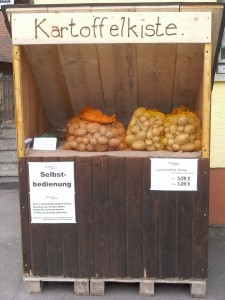
\includegraphics[width=0.3\textwidth,angle=0]{abb/Kartoffelkiste}
	\caption[Die Kartoffelkiste]{\glqq Kartoffelkiste\grqq{} \cite{Kartoffelkiste}}
	\label{fig:Kartoffelkiste}
\end{figure}


\begin{figure}[hh]
	\centering
	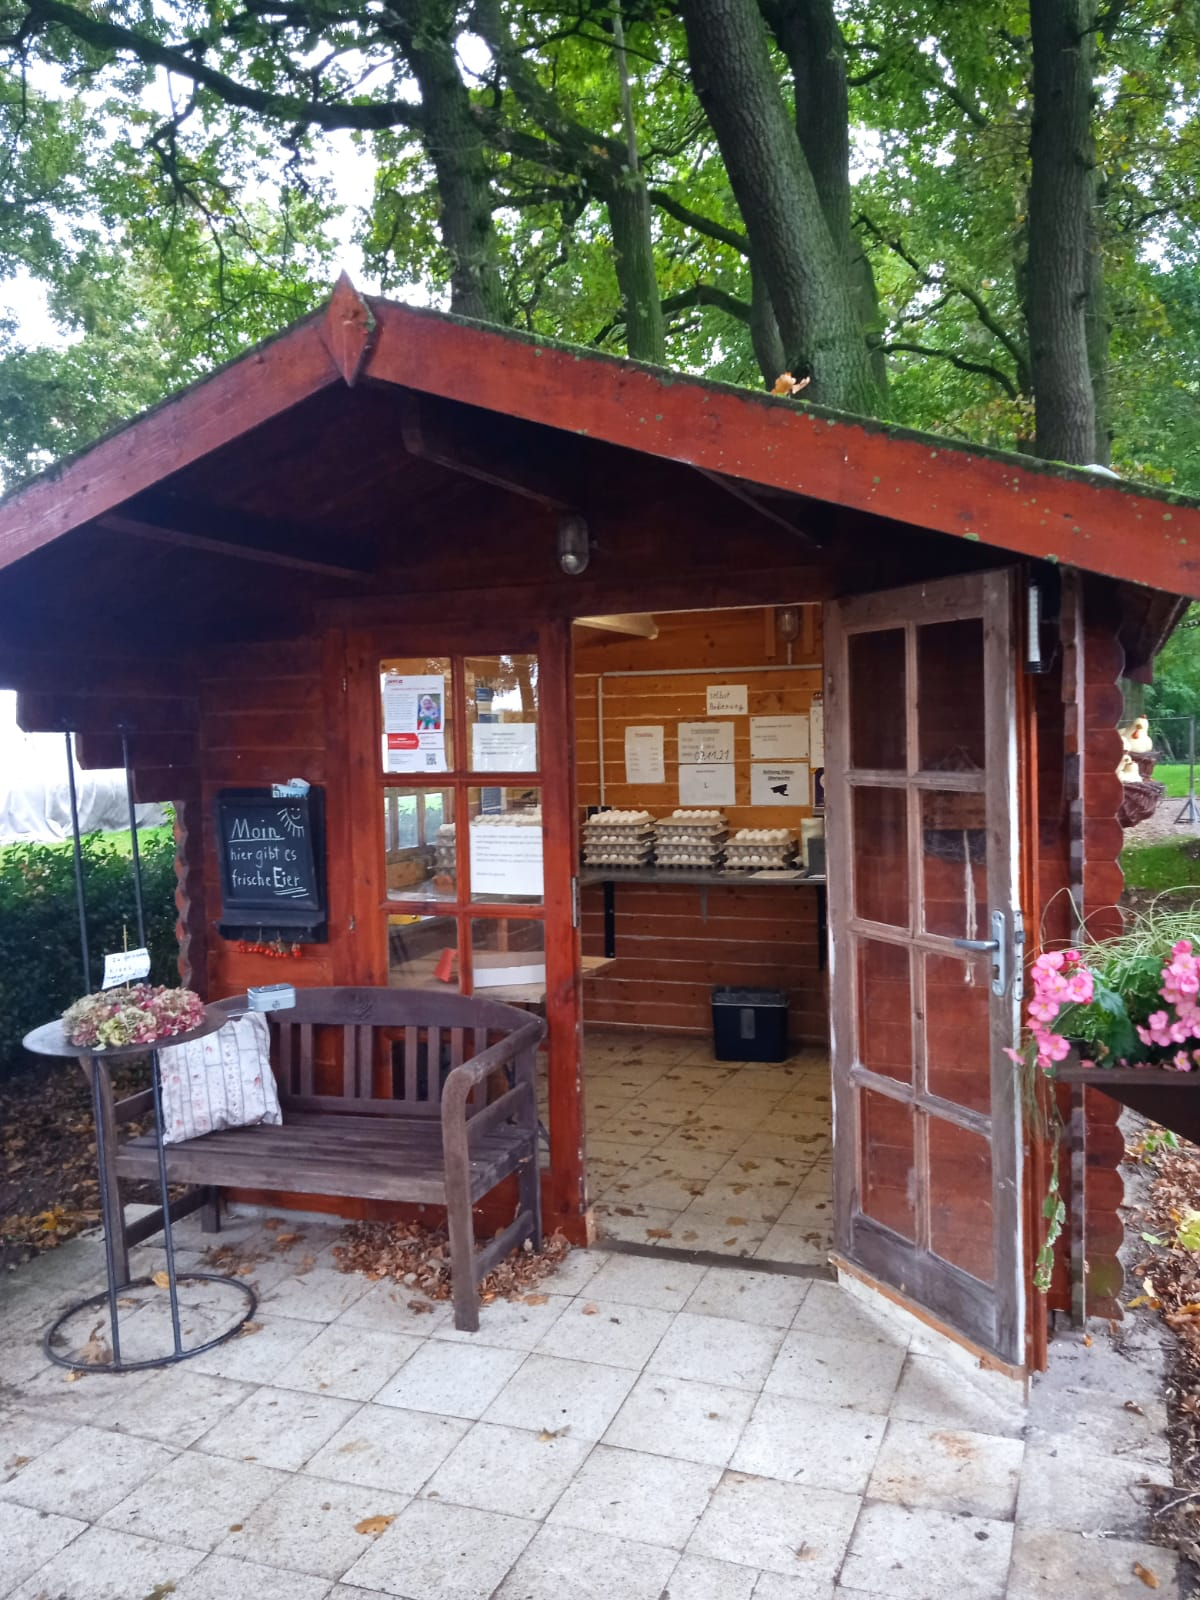
\includegraphics[width=0.3\textwidth,angle=0]{abb/Eierhaus}
	\caption[Eierhaus]{Eierhaus }
	\label{fig:Eierhaus}
\end{figure}


Der Begriff Selbstbedienung wird von \cite{Selbstbedienung} wie folgt definiert \glqq Verkaufsprinzip im Handel, bei dem der Kunde aus einem frei zugänglichen und griffbereit ausgestellten Warensortiment ohne Mitwirkung des Verkaufspersonals die von ihm gewählten Artikel zu den betrieblichen Inkassostellen transportiert.\grqq{} 
\\
\\
\\
Bei einem Kauf in einer Selbstbedienungshütte bezahlt der Kunde seine Ware 
selbstständig, ohne Verkaufspersonal und wirft das Geld in einen dafür vorgesehenen Behälter. Dieses kann zum Beispiel eine abschließbare Geldkassette mit Münzeinwurf sein.
\\
Der Stand bzw. der Ort, an dem die Waren angeboten werden, kann die unterschiedlichsten Bauweisen oder Formen aufweisen.

Auf dem Bild~\ref{fig:Kartoffelkiste} und dem Bild~\ref{fig:Eierhaus} sind zwei unterschiedliche Bauweisen zu sehen. Das Bild~\ref{fig:Kartoffelkiste} zeigt einen Straßenstand, auf dem zweiten Bild~\ref{fig:Eierhaus} ist eine Blockhütte zu sehen.


\subsection{Gesetzliche Grundlagen}\label{gesetzliche Grundlagen}

In diesem Kapitel werden einige gesetzliche Grundlagen vorgestellt. 
Es ist nicht möglich auf alle gesetzlichen Vorschriften einzugehen, da es zu viele unterschiedliche Reglungen gibt.
Außerdem werden die hier vorgestellten Vorschriften und Reglungen nicht im Detail erläutert. Für ausführlichere Informationen muss der Betreiber sich bei den zuständigen Stellen erkundigen. 
\\
\\
Als Erstes wird geklärt, was Direktvermarktung landwirtschaftlicher Erzeugnisse eigentlich bedeutet. \cite{gesetze1} schreibt \glqq Unter Direktvermarktung
versteht man die direkte Abgabe landwirtschaftlicher Produkte durch den Erzeuger auf dem Hof, auf dem Markt, an der Tür oder über eigene Hofläden an den Verbraucher.\grqq{} 
\\
\\
Werden nur \glqq selbsterzeugte unverarbeitete landwirtschaftliche Produkte, die als Urprodukte gelten vermarktet\grqq{}, ist dieses \glqq kein Gewerbe im Sinne der Gewerbeordnung\grqq{} erwähnt \cite{gesetze4}. Außerdem heißt es dort weiter \glqq werden (Ur-)Produkte für den Verkauf gereinigt, sortiert und hergerichtet (sogenannte erste Verarbeitungsstufe), so ist dies unschädlich.\grqq{}
\\
\\
\begin{table}[h]
	\centering
	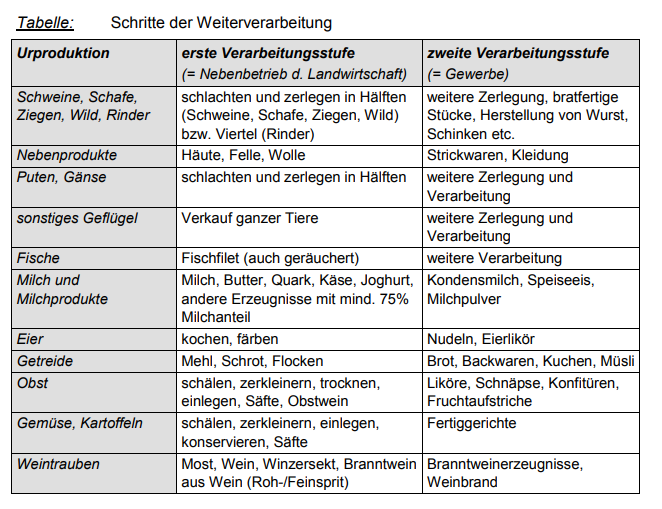
\includegraphics[width=0.8\textwidth,angle=0]{abb/urproduktion}
	\caption[Urproduktion, Schritte der Weiterverarbeitung]{Urproduktion, \glqq Schritte der Weiterverarbeitung\grqq{} \cite{gesetze2}}
	\label{tab:Urproduktion}
\end{table}


In der Tabelle~\ref{tab:Urproduktion} sind einige Urprodukte der ersten und zweiten Verarbeitungsstufe abgebildet. 
\\
Folgende Punkte führen zur Anzeigepflicht eines Gewerbes:\cite{gesetze2}


\begin{itemize}
	\item Der Verkauf von weiterverarbeiteten Produkten (zweite Verarbeitungsstufe) erzielt einen Umsatz von 10 Prozent des Gesamtumsatzes oder mehr des Betriebes.
	\item Verkauf von zugekaufter Ware, deren Umsatz 10 Prozent oder mehr des Betriebsumsatzes ausmachen.
	\item Verkauf und Urproduktion sind räumlich und personell getrennt. Ausgenommen hiervon ist ist der Marktstand.
\end{itemize}


Eine Vertrauenskasse wird laut \cite{gesetze5} wie folgt definiert \glqq Kasse, in die der Käufer selbständig den Kaufbetrag für die gekaufte Ware oder Leistung einzahlt, ohne dass in irgendeiner anderen Form der Verkäufer kassiert\grqq{}.
\\
\\
\cite{Bundesministerium} schreibt \glqq Als offene Ladenkasse gelten eine summarische, retrograde Ermittlung der Tageseinnahmen sowie manuelle Einzelaufzeichnungen ohne Einsatz technischer Hilfsmittel (BMF-Schreiben v. 19.6.2018).\grqq{} 
Der Begriff offene Ladenkasse bezieht sich nicht auf die Bauform der Kasse, sondern auf die Art, wie die Tageseinnahmen ermittelt werden.
\\ 
\\
Ein Landwirt, der direkt seine Produkte vermarktet, muss alle Einnahmen aufzeichnen. Diese müssen \glqq in einem Kassenbericht vollständig, richtig, zeitgerecht und geordnet aufgezeichnet werden\grqq{}, erwähnt \cite{gesetze7}. Dort heißt es weiter \glqq Laut Gesetz kommt bei Bargeldgeschäften der Grundsatz der Einzelauszeichnung zur Anwendung, [...] Da dieser Grundsatz in einem Hofladen [...] nicht praktikabel ist, gelten bestimmte Vereinfachungen.\grqq{} Diese Vereinfachungen besagen das es reicht, täglich die Summer der verkauften Waren und deren Einnahmen zu protokollieren.

\begin{table}[htb]
	\centering
	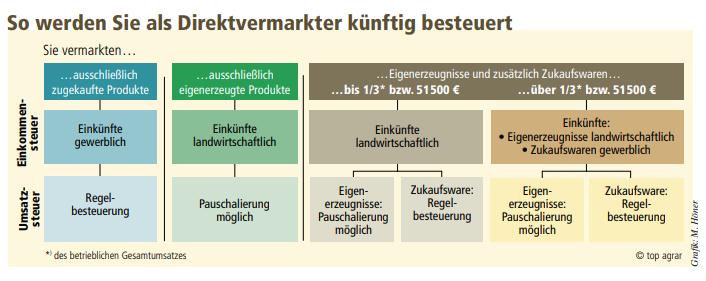
\includegraphics[width=1\textwidth,angle=0]{abb/versteuerung}
	\caption[Übersicht, Versteuerung Direktvermarkter]{Übersicht, Versteuerung Direktvermarkter \cite{gesetze3}}
	\label{fig:versteuerung}
\end{table}


In der Tabelle~\ref{fig:versteuerung} sind mögliche Versteuerungen zu sehen. Wichtig zu wissen, dies ist nur eine Übersicht, es kann möglicherweise sein, dass es im Steuerrecht abweichende Grenzen und Regeln gibt.
\\
\\
Nachfolgend werden ein paar weitere gesetzliche Reglungen aufgezählt, die eventuell beachtet werden müssen: Handwerksordnung, Gewerbeordnung, Steuerrecht, Baurecht, Lebensmittelhygienerecht, Qualitätskennzeichen, Verpackungsgesetz usw..


\subsection{Begriffsdefinitionen und Begriffserklärung}\label{begriffsdefinitionen}
Dieses Kapitel soll einen Überblick über verwendete Begriffsdefinitionen geben, zusätzlich werden einige Begriffe etwas genauer beschrieben.

\subsubsection{Client-Server-Architektur}\label{client-Server-Architektur}

Zunächst wird dargestellt, was ein Server ist, anschließend wird auf den Client eingegangen.
\\
\\
Laut \cite{clientServerModel} sind Server und Client keine reinen Hardwarekomponenten, sondern der Begriff \glqq Server und Client\grqq{} beschreibt Rollen.
\\
\\
\cite{clientServerModel} stellt fest das die Aufgabe eines Servers daraus besteht \glqq einen bestimmten Dienst lokal oder über das Netzwerk bereitzustellen.\grqq{}
Ein Server kann zum Beispiel Daten, Anwendungen, Dienste usw. bereitstellen. 
\\
\cite{win08}~[S.116] schreibt \glqq Eine Hardware- oder Softwarekomponente, der Dienste von einem Server in Anspruch nehmen kann (Client-Server-Prinzip) wird Client (Kunde) genannt.\grqq{} Dieses könnte zum Beispiel ein Computer sein, der die Dienste eines Servers in Anspruch nimmt. 
\\
Der Autor \cite{clientServerModel} erwähnt \glqq Das Client-Server-Modell ist ein Architekturkonzept zur Verteilung von Diensten und Aufgaben in einem Netzwerk. Dienste werden von Servern bereitgestellt und können von Clients genutzt werden.\grqq{}.

\begin{figure}[htb]
	\centering
	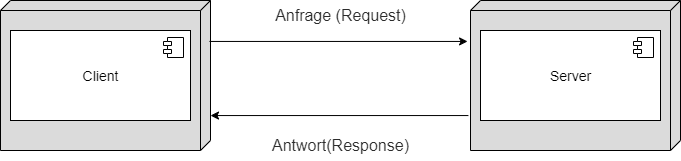
\includegraphics[width=1\textwidth,angle=0]{abb/Client-Server-Grundlagen}
	\caption[Vereinfachte Darstellung einer Kommunikation zwischen Client und Server]{Vereinfachte Darstellung einer Kommunikation \\ zwischen Client und Server}
	\label{fig:AB_Client-Server-Kommunikation_Grundlagen}
\end{figure}

Die Abbildung~\ref{fig:AB_Client-Server-Kommunikation_Grundlagen} stellt eine vereinfachte Darstellung einer Kommunikation zwischen Client und Server dar. Ein Client sendet eine Anfrage (Request) an einen Server, dieser verarbeitet die Anfrage und schickt eine Antwort (Response) zurück an den Client. Durchaus mehrere Clients können auf einen Server zugreifen. Außerdem kann sowohl der Client und der Server auf den selben Rechner ausgeführt werden.
\\
\cite{clientServerModel} schreibt, dass die Kommunikation und der Informationsaustausch über Protokolle geregelt wird. Bekannte und häufig verwendete Protokolle sind laut \cite{clientServerModel} das \glqq FTP (File Transfer Protokoll), HTTP (Hypertext Transfer Protocol) und das SNMP (Simple Network Management Protocol)\grqq{}.
\\
Ein Server baut nicht selbstständig eine Verbindung auf, sondern wartet auf eine Verbindungsanfrage.
\\
Ein typisches Beispiel einer Client-Server-Architektur ist ein Webbrowser, der auf einem Client läuft, dieser sendet eine Anfrage an einen Webserver und möchte eine bestimmte Internetseite aufrufen. Der Server prüft diese Anfrage und sendet die gewünschten Daten zurück.
\\
Einer der am häufigsten genutzten Webservern, ist der Apache HTTP Server\footnote{https://httpd.apache.org}. 

\subsubsection{REST-API}\label{RestAPI}

REST-API ist die Abkürzung von \glqq Representational State Transfer - Application Programming Interface \grqq{} beschreibt \cite{RESTAPI}.
Eine REST-API ist eine Programmierschnittstelle, mithilfe einer Schnittstelle ist es möglich, Daten und Informationen zwischen unterschiedlichen Systemen auszutauschen.
Der Autor \cite{RESTAPI2} erklärt \glqq Der als REST (oder auch ReST) bezeichnete Architekturansatz beschreibt, wie verteilte Systeme miteinander kommunizieren können.\grqq{}.
Gemäß \cite{RESTAPI} werden HTTP-Anfrage genutzt um auf Informationen zuzugreifen.
Die bekanntesten oft genutzte HTTP-Anfragen sind: \cite{RESTAPI2}

\begin{itemize}
	\itemsep0pt
	\item GET - Der Client fordert Daten vom Server an.
	\item POST - Der Server sendet die angeforderten Daten an den Client.
	\item PUT/PATCH - Der Server ändert vorhandene Daten.
	\item DELETE - Es sollen Daten vom Server gelöscht werden.
\end{itemize}

Schreibt das \cite{horn} alternativ auch das Nachrichtenprotokoll SOAP (Simple Object Access Protocol) verwendet werden kann.
\\
\\
\glqq Die Antworten werden oft im JSON-Format (JavaScript Object Notation) geliefert. Das Format ist sowohl für Menschen als auch Maschinen lesbar.\grqq{} berichtet \cite{RESTAPI3}.
\\
\lstset{language=java}
\begin{lstlisting}[frame=htrbl, caption={Beispiel für Daten im JSON Format}, label={lst:JSON}]
{
	"Benutzer": {
		"Name": [
		{
			"id": 1,
			"Vorname": "Christine",
			"Nachname": "Dall",
			"Administrator": true,
			"Adresse": null
		},
		{
			"id": 2,
			"Vorname": "Christin",
			"Nachname": "Ball",
			"Administrator": false,
			"Adresse": "Neuer Weg 6, 12345 Ort"
		},
		{
			"id": 3,
			"Vorname": "Christina",
			"Nachname": "Fall",
			"Administrator": false,
			"Adresse": null
		}
		]
	}
}
\end{lstlisting}

Im Listing~\ref{lst:JSON} zu sehen ist eine beispielhafte Datenstruktur. Dieses könnten zum Beispiel Daten, sein die der Client über eine Get-Anfrage erhält.
\\
\\
Außerdem wird vom Server auf jede Anfrage ein HTTP-Statuscode mitgesendet. Bekannte Statuscodes sind unter anderem: \cite{Statuscodes}
\begin{itemize}
	\itemsep0pt
	\item 200, OK
	\item 201, Erzeugt
	\item 400, Ungültige Anfrage
	\item 403, Verboten
	\item 404, Nicht gefunden
	\item 408, Anfrage-Zeitüberschreitung
	\item 409, Konflikt
	\item 500, Interner Server-Fehler
\end{itemize}

\subsubsection{Frameworks zur Realisierung einer Client-Server-Architektur}\label{frameworks zur Realisierung einer Client-Server-Architektur}

Ein Framework ist ein Programmiergerüst, dieses wird überwiegend in der objektorientierten Programmierung eingesetzt, dieses bildet den Rahmen und Anwendungsarchitektur einer Anwendung definiert \cite{Framework1}. Weiter heißt es dort \glqq Das Framework umfasst Bibliotheken, Komponenten und Laufzeitumgebungen und stellt die Designgrundstruktur für die Entwicklung zur Verfügung.\grqq{}.
\\
\\
Die Arbeit mit Frameworks bietet einige Vorteile. \cite{Framework2} erwähnt folgenden Vorteil, \glqq Wiederkehrende Aufgaben können schneller abgewickelt werden,\grqq{} bei der Verwendung von Frameworks spart sich der Programmierer Zeit und Aufwand.
\\
\\
Nachfolgend werden ein paar Frameworks und eine Bibliothek vorgestellt. 
\\
\\
\\
\\
\\
\\
Der Unterschied zwischen Bibliotheken und Frameworks ist \glqq Bei einer Bibliothek handelt es sich um eine Sammlung von Programmroutinen, die oft einen thematischen Zusammenhang aufweisen.\grqq{} schreibt \cite{AngularReactVergleich12}. Bibliotheken ergänzen Programmiersprachen um Funktionen. Ein Framework ist ein universelles Rahmenwerk und \glqq Um dieses rasch und übersichtlich einsetzen zu können, verwendet es nicht selten eine ergänzte oder variierte Syntax beziehungsweise eine eigene Programmiersprache und Struktur.\grqq{} wird noch ergänzend geschrieben von \cite{AngularReactVergleich12}. 
\\
\\
Vorgestellt werden Angular, React, Vue.js und Spring Boot. 
\\

\begin{longtable}{|l|l|l|}
	\hline
\rowcolor[gray]{0.6}	 & \multicolumn{2}{p{9.0cm}|}{ \textbf{Angular}} \\
\hline
	\hline
	Typ & \multicolumn{2}{l|}{Web-Framework } \\
	\hline
	Veröffentlichung & \multicolumn{2}{l|}{2016 entwickelt von Google Inc. \cite{AngularReactVergleich}} \\
	\hline
	Aktuelle Version & \multicolumn{2}{l|}{Angular 12.1.1 (Stand: 30.06.2021) } \\
	\hline
	Lizenz & \multicolumn{2}{l|}{MIT-Lizenz} \\
	\hline
	Betriebssystem & \multicolumn{2}{l|}{Plattformunabhängig} \\
	\hline
	Programmiersprache & \multicolumn{2}{l|}{TypeScript} \\
	\hline
	Webseiten die Angular nutzen & \multicolumn{2}{l|}{Youtube, PayPal} \\
	\hline
	\hline
	\multicolumn{3}{|p{14.0cm}|}{
	Bemerkung
	
Angular ist der Nachfolger von AngularJS und wurde komplett neu geschrieben. 

Der Autor \cite{AngularReactVergleich5} erwähnt das mit Angular komponentenbasiert entwickelt wird. 
		
	Eine Komponente besteht aus: \cite{AngularReactVergleich5}
	\begin{itemize}
		\itemsep0pt
		\item Template, enthält das HTML-Grundgerüst.
		\item Klasse, enthält die Logik die das Verhalten der Komponente steuert.
		\item Stylesheet, enthält das Layout.
	\end{itemize}
	} \\
	\hline
	\hline
	\multicolumn{3}{|p{12.0cm}|}{
		Vorteile
	
	\begin{itemize}
		\itemsep0pt
		\item Große Community \cite{AngularReactVergleich2}
		\item Große Typsicherheit, da TypeScript verwendet wird. \cite{AngularReactVergleich3}
		\item Erfordert keine zusätzlichen Bibliotheken \cite{AngularReactVergleich2}.
		\item \glqq Komponentenbasierte Architektur\grqq{} \cite{AngularReactVergleich5}
		\item Große Wiederverwendbarkeit der Komponenten \cite{AngularReactVergleich4}
		\item \glqq Zukunftssicher\grqq{} \cite{AngularReactVergleich5}
		\item Stabiles und verlässliches Framework \cite{AngularReactVergleich6}
		\item Hohe Performance. \cite{AngularReactVergleich5}
		\item Gut bei anspruchsvollen Backend-Anwendungen. \cite{AngularReactVergleich2}
		\item Verwendet HTML, CSS, Javascript, dieses ist vielen Entwicklern bereits bekannt. \cite{AngularReactVergleich3}
		\item Enthält viele Features (\glqq Dependency Injection, Templates, Routing, Ajax Requests\grqq{} \cite{AngularReactVergleich})
		\item Gute Dokumentation
	\end{itemize}} \\
	\hline
	\hline
	\multicolumn{3}{|p{12.0cm}|}{Nachteile
	
\begin{itemize}
	\itemsep0pt
	\item Hohe Einstiegshürde \cite{AngularReactVergleich2}
	\item Komplexes Framework \cite{AngularReactVergleich4}
	\item Abnehmender Community Support \cite{AngularReactVergleich4}
	\item Angular Versionen sind wenig kompatibel untereinander. \cite{AngularReactVergleich6}
	\item Geringere Flexibilität  \cite{AngularReactVergleich}
\end{itemize}} \\
	\hline
	\caption{Vorstellung des Frameworks Angular}
	\label{tab:dlsc}
\end{longtable}



\newpage


\begin{longtable}{|l|l|l|}
	\hline
	\rowcolor[gray]{0.6}	 & \multicolumn{2}{p{9.0cm}|}{ \textbf{React}} \\
	\hline
	Typ & \multicolumn{2}{l|}{JavaScript-Bibliothek} \\
	\hline
	Veröffentlichung & \multicolumn{2}{l|}{2013 entwickelt von Facebook Inc. \cite{AngularReactVergleich}} \\
	\hline
	Aktuelle Version & \multicolumn{2}{l|}{17.0.02 (Stand: 30.06.2021)  } \\
	\hline
	Lizenz & \multicolumn{2}{l|}{MIT-Lizenz} \\
	\hline
	Betriebssystem & \multicolumn{2}{l|}{Plattformunabhängig (Ab Version 3)} \\
	\hline
	Programmiersprache & \multicolumn{2}{l|}{JavaScript, ab Version 3 auch TypeScript } \\
	\hline
	Webseiten die React nutzen & \multicolumn{2}{l|}{Facebook, Instagram, Discord, Pinterest} \\
	\hline
	\hline
	\multicolumn{3}{|p{14.0cm}|}{
		Bemerkung
		
\cite{AngularReactVergleich} schreibt React besteht nur aus der 
View-Komponente. Diese Komponente beinhaltet \glqq den UI-Teil und die Logik der Applikation\grqq{}.
	
	} \\
	\hline
	\hline
	\multicolumn{3}{|p{12.0cm}|}{
		Vorteile
		
	\begin{itemize}
		\itemsep0pt
		\item Virtuelles DOM (Document Object Model), Veränderungen am eigentlich DOM werden dadurch klein gehalten. \cite{AngularReactVergleich3}
		\item Große Flexibilität \cite{AngularReactVergleich4}
		\item \glqq schlank, klein und elementar gehalten\grqq{} am Anfang sind nur Grundfunktionen verfügbar. \cite{AngularReactVergleich7}
		\item Beliebt, dadurch große Community vorhanden\cite{AngularReactVergleich4}
		\item Keine so hohe Einstiegshürde wie Angular. \cite{AngularReactVergleich3}
		\item Gute Unterstützung interaktiver Elemente. \cite{AngularReactVergleich2}
		\item Gute Dokumentation
		\item Es werden regelmäßig Updates veröffentlicht. 
	\end{itemize}} \\
	\hline
	\hline
	\multicolumn{3}{|p{12.0cm}|}{Nachteile
		
	\begin{itemize}
		\itemsep0pt
		\item Erfordert eventuell zusätzliche Bibliotheken. \cite{AngularReactVergleich}
		\item Wenig Futures, benötigte Packages müssen nachinstalliert werden. \cite{AngularReactVergleich}
		\item Template wird mit JSX geschrieben, Sprache muss eventuell gelernt werden. \cite{AngularReactVergleich7}
		\item Der Einsatz lohnt sich nur für Seiten die viele Interaktive Elemente enthalten. \cite{AngularReactVergleich3}
	\end{itemize}} \\
	\hline
		\caption{Vorstellung der Bibliothek React}
	\label{tab:react}
\end{longtable}





\begin{longtable}{|l|l|l|}
	\hline
	\rowcolor[gray]{0.6}	 & \multicolumn{2}{p{9.0cm}|}{ \textbf{Vue.js}} \\
	\hline
	Typ & \multicolumn{2}{l|}{Web-Framework} \\
	\hline
	Veröffentlichung & \multicolumn{2}{l|}{2014 entwickelt Evan You \cite{AngularReactVergleich}} \\
	\hline
	Aktuelle Version & \multicolumn{2}{l|}{17.0.02 (Stand: 30.06.2021)  } \\
	\hline
	Lizenz & \multicolumn{2}{l|}{MIT-Lizenz} \\
	\hline
	Betriebssystem & \multicolumn{2}{l|}{Plattformunabhängig (Ab Version 3)} \\
	\hline
	Programmiersprache & \multicolumn{2}{l|}{JavaScript, ab Version 3 auch TypeScript } \\
	\hline
	Webseiten die Vue.js nutzen & \multicolumn{2}{l|}{Gitlab, Nintendo, Shopware} \\
	\hline
	\hline
	\multicolumn{3}{|p{14.0cm}|}{
Bemerkung
		
Bei Vue.js\glqq handelt es sich hier um eine monolithische Lösung, die dem Entwickler alle nötigen Tools für eine umfassende Applikation anbietet.\grqq{} \cite{AngularReactVergleich7}
	} \\
	\hline
	\hline
	\multicolumn{3}{|p{12.0cm}|}{
		Vorteile
		
	\begin{itemize}
		\itemsep0pt
		\item Leichter Einsieg \cite{AngularReactVergleich8}
		\item Modularer Aufbau  \cite{AngularReactVergleich9}
		\item Schlanker Aufbau, unterschiedliche Module können hinzugefügt werden.\cite{AngularReactVergleich10} 
		\item \glqq 50 \% weniger Renderzeit: im Vergleich zu anderen Frameworks.\grqq{}\cite{AngularReactVergleich11}
		\item Virtuelles DOM (Document Object Model), Veränderungen am eigentlich DOM werden dadurch klein gehalten. \cite{AngularReactVergleich9}
		\item Ist nur 10 kB groß.(Version 3) \cite{AngularReactVergleich11}
	\end{itemize}} \\
	\hline
	\hline
	\multicolumn{3}{|p{12.0cm}|}{Nachteile
		
	\begin{itemize}
		\itemsep0pt
		\item Kleine Community \cite{AngularReactVergleich4}
		\item Kleines Entwicklerteam \cite{AngularReactVergleich9}
		\item Wenig Erweiterungen. \cite{AngularReactVergleich12}
	\end{itemize}} \\
	\hline
		\caption{Vorstellung des Frameworks Vue.js}
	\label{tab:vue}
\end{longtable}


\newpage

\begin{longtable}{|l|l|l|}
	\hline
	\rowcolor[gray]{0.6} & \multicolumn{2}{p{9.0cm}|}{ \textbf{Spring Boot}} \\
	\hline
	Typ & \multicolumn{2}{l|}{Application Framework} \\
	\hline
	Veröffentlichung & \multicolumn{2}{l|}{2002 entwickelt von Rod Johnson, ab September 2009 VMware} \\
	\hline
	Aktuelle Version & \multicolumn{2}{l|}{ 5.3.8 (Stand: 30.06.2021)  } \\
	\hline
	Lizenz & \multicolumn{2}{l|}{Apache-Lizenz} \\
	\hline
	Programmiersprache & \multicolumn{2}{l|}{Java, Kotlin, Groovy } \\
	\hline
	\multicolumn{3}{|p{14.0cm}|}{
		Bemerkung
				
\cite{Spring2} definiert \glqq Das Spring Framework ist ein schlankes Open-Source-Framework für Java. Mittels Dependency Injection und aspektorientierter Programmierung soll es einen insgesamt leichteren und besser wartbaren Programmcode ermöglicht.\grqq{}
	} \\
	\hline
	\hline
	\multicolumn{3}{|p{12.0cm}|}{
		Vorteile
		
		\begin{itemize}
		\itemsep0pt
		\item MVC-Architektur
		\item Dependency Injection
		\item Aspektorientierte Programmierung 
		\item Flexible Modulsammlung 
		\item Große Community
		\item Ausführliche Dokumentation
		\item Flache Lernkurve \cite{Spring3}
		\item Unterstützt viele Datenbanken  \cite{Spring3}
	\end{itemize}} \\
	\hline
	\hline
	\multicolumn{3}{|p{12.0cm}|}{Nachteile
		
	\begin{itemize}
		\itemsep0pt
		\item Höhere Code-Ausführungszeit
		\item Erfordert Einarbeitungszeit
	\end{itemize}} \\
	\hline
		\caption{Vorstellung des Frameworks Spring Boot}
	\label{tab:spring}
\end{longtable}

\subsection{SQL-Datenbank}\label{sQL-Datenbank}
Datenbanken werden in fast jeder größeren Softwareanwendung in der IT verwendet. 
In einer Datenbank werden Daten bereitgestellt und gespeichert, die für den Betrieb der Software nötig sind.
Das können zum Beispiel folgende Daten sein: Benutzername, Passwort, Artikelinformationen usw..
\\
\\
\\
Gemäß \cite{win08} ~[S.55] ist eine Datenbank, eine strukturierte, dauerhaft elektronisch gespeicherte Sammlung von Datenmengen. Eine Datenbank kann mithilfe eines Datenbankmanagementsystems (DBMS) verwaltet werden. Bekannte DBMS sind unter anderem MySQL\footnote{https://www.mysql.com/de/} und Oracle\footnote{https://www.oracle.com/database/}. 
\\
\\
In der Praxis werden unterschiedliche Datenbankmodell verwendet, eines der am häufigsten genutzten Systeme ist das relationale Datenbankmodell. 
\cite{t3rationaleDatenbank} schreibt, dass eine relationale Datenbank aus unterschiedlich vielen Tabellen bestehen kann. Es werden logisch zusammenhängende Daten miteinander verknüpft (in Relation gesetzt). \cite{oracleDB} beschreibt eine relationale Datenbank als \glqq ein Typ von Datenbanken, der die Speicherung und den Zugriff auf miteinander verbundener Datenpunkte ermöglicht.\grqq{}.
\\
\\
Mithilfe einer Datenbanksprache lassen sich unter anderem Daten einfügen, löschen oder verändern. Diese Datenbankoperationen sind auch unter dem Begriff CRUD bekannt. \cite{db2222} erklärt das die Abkürzung sich aus den Begriffen Create, Read, Update, Delete zusammensetzt.
\\
\\
In dieser Praxisarbeit wird SQL verwendet, die Abkürzung steht für Structured Query Language. Gemäß \cite{datenbankenVerstehen} ist SQL \glqq eine Datenbanksprache zur Erstellung von Datenbankstrukturen in relationalen Datenbanken sowie zum Bearbeiten und Abfragen der darauf basierenden Datenbeständen.\grqq{}.
\\
\cite{Lub17} erwähnt das SQL keine vollwertige Programmiersprache ist, das heißt hiermit können keine kompletten Anwendungen erstellt werden, aber SQL lässt sich gut mit Programmiersprachen kombinieren. \cite{bitfarm} schreibt das SQL, durch die weite Verbreitung zum Standard in Deutschland geworden ist.
\\
\\
Laut \cite{Lub17} lassen sich die SQL-Befehle in drei unterschiedliche Kategorien aufteilen.
Die drei Kategorien sind, DML-Befehle (Data Manipulation Language Befehle), DDL-Befehle (Data Definition Language Befehle) und DCL-Befehle (Data Control Language Befehle).
\\
DML-Befehle werden zum Bearbeiten, Löschen und Einfügen verwendet. Bekannte und oft verwendete Befehle werden in der Tabelle~\ref{tab:dml} dargestellt.
\\
DDL-Befehle sind dazu geeignet, die Struktur der Datenbank zu steuern.
Bekannte DDL-Befehle sind in der Tabelle~\ref{tab:ddl} abgebildet.
\\
Außerdem gibt es noch die DLC-Befehle, diese Befehle helfen bei der Rechteverwaltung. Beispiele hierfür sind in der Tabelle~\ref{tab:dlc} zusehen. 
\\
\\
\\
In den nachfolgenden Tabellen werden einige Beispielbefehle, entnommen aus \cite{w3SQL}, aufgezeigt.
\\
\\
\begin{table}[h]
	\begin{tabular}{|p{7cm}|p{7cm}|}
		\hline
		\textbf{Befehl} & \textbf{Beschreibung} \\
		\hline
		SELECT * FROM Tabellenname & Mit diesem Befehl werden Daten aus Tabellen ausgelesen. \\
		\hline
		INSERT INTO Tabellenname (Spaltenname1, Spaltenname2, ... ) VALUES (Wert1, Wert 2, ...)	 & Dieser Befehl fügt Daten in die Tabelle ein. \\
		\hline
		DELETE FROM Tabellenname WHERE Bedienung & Mithilfe dieses Befehls werden Daten aus der Tabelle gelöscht. \\
		\hline
		UPDATE Tabellenname SET (Spalte1 = Wert1, Spalte2 = Wert2, ...) WHERE Bedienung  & Dieser Befehl sorgt dafür, dass Daten in der Tabelle aktualisiert werden. \\
		\hline
	\end{tabular}
	\caption{DML-Befehle}
	\label{tab:dml}
\end{table}
\\  

\begin{table}[h]
	\begin{tabular}{|p{7cm}|p{7cm}|}
		\hline
		\textbf{Befehl} & \textbf{Beschreibung} \\
		\hline
		CREATE DATABASE Datenbankname & Mithilfe dieses Befehls wird eine neue Datenbank erstellt. \\
		\hline
		CREATE TABLE Tabellenname (Spaltenname1 Datentyp1, Spaltenname2 Datentyp2, ...) & Dieser Befehl sorgt dafür, dass eine neue Tabelle angelegt wird.\\
		\hline
		DROP TABLE Tabellenname & Soll eine Tabelle gelöscht werden, kann dieser Befehl genutzt werden.\\
		\hline
		ALTER TABLE Tabellename ADD Spaltenname Datentyp & Es wird eine neue Spalte in der Tabelle eingefügt, sobald dieser Befehl genutzt wird. \\
		\hline
	\end{tabular}
	\caption{DDL-Befehle}
	\label{tab:ddl}
\end{table}


\begin{table}[h]
	\begin{tabular}{|p{7cm}|p{7cm}|}
		\hline
		\textbf{Befehl} & \textbf{Beschreibung} \\
		\hline
		GRANT Privileg  ON Datenbankname TO \{Benutzername |PUBLIC |Rollenname\}[WITH GRANT OPTION] & Die Zuggriffrechte werden mithilfe dieses Befehls gewährt. \\
		\hline
		REVOKE Privileg ON Datenbankname FROM \{Benutzername |PUBLIC |Rollenname\} &  Dieser Befehl entzieht dem Benutzer Zugriffsrechte.\\
		\hline
	\end{tabular}
	\caption{DLC-Befehle}
	\label{tab:dlc}
\end{table}
